\documentclass[twoside]{book}

% Packages required by doxygen
\usepackage{fixltx2e}
\usepackage{calc}
\usepackage{doxygen}
\usepackage[export]{adjustbox} % also loads graphicx
\usepackage{graphicx}
\usepackage[utf8]{inputenc}
\usepackage{makeidx}
\usepackage{multicol}
\usepackage{multirow}
\PassOptionsToPackage{warn}{textcomp}
\usepackage{textcomp}
\usepackage[nointegrals]{wasysym}
\usepackage[table]{xcolor}

% Font selection
\usepackage[T1]{fontenc}
\usepackage[scaled=.90]{helvet}
\usepackage{courier}
\usepackage{amssymb}
\usepackage{sectsty}
\renewcommand{\familydefault}{\sfdefault}
\allsectionsfont{%
  \fontseries{bc}\selectfont%
  \color{darkgray}%
}
\renewcommand{\DoxyLabelFont}{%
  \fontseries{bc}\selectfont%
  \color{darkgray}%
}
\newcommand{\+}{\discretionary{\mbox{\scriptsize$\hookleftarrow$}}{}{}}

% Page & text layout
\usepackage{geometry}
\geometry{%
  a4paper,%
  top=2.5cm,%
  bottom=2.5cm,%
  left=2.5cm,%
  right=2.5cm%
}
\tolerance=750
\hfuzz=15pt
\hbadness=750
\setlength{\emergencystretch}{15pt}
\setlength{\parindent}{0cm}
\setlength{\parskip}{3ex plus 2ex minus 2ex}
\makeatletter
\renewcommand{\paragraph}{%
  \@startsection{paragraph}{4}{0ex}{-1.0ex}{1.0ex}{%
    \normalfont\normalsize\bfseries\SS@parafont%
  }%
}
\renewcommand{\subparagraph}{%
  \@startsection{subparagraph}{5}{0ex}{-1.0ex}{1.0ex}{%
    \normalfont\normalsize\bfseries\SS@subparafont%
  }%
}
\makeatother

% Headers & footers
\usepackage{fancyhdr}
\pagestyle{fancyplain}
\fancyhead[LE]{\fancyplain{}{\bfseries\thepage}}
\fancyhead[CE]{\fancyplain{}{}}
\fancyhead[RE]{\fancyplain{}{\bfseries\leftmark}}
\fancyhead[LO]{\fancyplain{}{\bfseries\rightmark}}
\fancyhead[CO]{\fancyplain{}{}}
\fancyhead[RO]{\fancyplain{}{\bfseries\thepage}}
\fancyfoot[LE]{\fancyplain{}{}}
\fancyfoot[CE]{\fancyplain{}{}}
\fancyfoot[RE]{\fancyplain{}{\bfseries\scriptsize Generated by Doxygen }}
\fancyfoot[LO]{\fancyplain{}{\bfseries\scriptsize Generated by Doxygen }}
\fancyfoot[CO]{\fancyplain{}{}}
\fancyfoot[RO]{\fancyplain{}{}}
\renewcommand{\footrulewidth}{0.4pt}
\renewcommand{\chaptermark}[1]{%
  \markboth{#1}{}%
}
\renewcommand{\sectionmark}[1]{%
  \markright{\thesection\ #1}%
}

% Indices & bibliography
\usepackage{natbib}
\usepackage[titles]{tocloft}
\setcounter{tocdepth}{3}
\setcounter{secnumdepth}{5}
\makeindex

% Hyperlinks (required, but should be loaded last)
\usepackage{ifpdf}
\ifpdf
  \usepackage[pdftex,pagebackref=true]{hyperref}
\else
  \usepackage[ps2pdf,pagebackref=true]{hyperref}
\fi
\hypersetup{%
  colorlinks=true,%
  linkcolor=blue,%
  citecolor=blue,%
  unicode%
}

% Custom commands
\newcommand{\clearemptydoublepage}{%
  \newpage{\pagestyle{empty}\cleardoublepage}%
}

\usepackage{caption}
\captionsetup{labelsep=space,justification=centering,font={bf},singlelinecheck=off,skip=4pt,position=top}

%===== C O N T E N T S =====

\begin{document}

% Titlepage & ToC
\hypersetup{pageanchor=false,
             bookmarksnumbered=true,
             pdfencoding=unicode
            }
\pagenumbering{roman}
\begin{titlepage}
\vspace*{7cm}
\begin{center}%
{\Large Position Based Fluids }\\
\vspace*{1cm}
{\large Generated by Doxygen 1.8.11}\\
\end{center}
\end{titlepage}
\clearemptydoublepage
\tableofcontents
\clearemptydoublepage
\pagenumbering{arabic}
\hypersetup{pageanchor=true}

%--- Begin generated contents ---
\chapter{Todo List}
\label{todo}
\hypertarget{todo}{}

\begin{DoxyRefList}
\item[\label{todo__todo000001}%
\hypertarget{todo__todo000001}{}%
File \hyperlink{BoundingBox_8h}{Bounding\+Box.h} ]Add the possibility to define each corner point for non axis-\/aligned boxes.  
\item[\label{todo__todo000002}%
\hypertarget{todo__todo000002}{}%
File \hyperlink{FluidSolver_8h}{Fluid\+Solver.h} ]Make the code more robust  
\item[\label{todo__todo000003}%
\hypertarget{todo__todo000003}{}%
File \hyperlink{FluidSystem_8h}{Fluid\+System.h} ]Implement a G\+UI to run the variables in the system  
\item[\label{todo__todo000004}%
\hypertarget{todo__todo000004}{}%
File \hyperlink{NNS_8h}{N\+NS.h} ]Research and implement a more efficient way  
\item[\label{todo__todo000005}%
\hypertarget{todo__todo000005}{}%
File \hyperlink{Particle_8h}{Particle.h} ]Refining 
\end{DoxyRefList}
\chapter{Hierarchical Index}
\section{Class Hierarchy}
This inheritance list is sorted roughly, but not completely, alphabetically\+:\begin{DoxyCompactList}
\item \contentsline{section}{Bounding\+Box}{\pageref{classBoundingBox}}{}
\item \contentsline{section}{Fluid\+Solver}{\pageref{classFluidSolver}}{}
\item \contentsline{section}{Fluid\+System}{\pageref{classFluidSystem}}{}
\item \contentsline{section}{N\+NS}{\pageref{classNNS}}{}
\item \contentsline{section}{Particle}{\pageref{structParticle}}{}
\item Q\+Open\+G\+L\+Window\begin{DoxyCompactList}
\item \contentsline{section}{N\+G\+L\+Scene}{\pageref{classNGLScene}}{}
\end{DoxyCompactList}
\item \contentsline{section}{Wall}{\pageref{structWall}}{}
\end{DoxyCompactList}

\chapter{Class Index}
\section{Class List}
Here are the classes, structs, unions and interfaces with brief descriptions\+:\begin{DoxyCompactList}
\item\contentsline{section}{\hyperlink{classBoundingBox}{Bounding\+Box} \\*Simple \hyperlink{classBoundingBox}{Bounding\+Box} class to work as the boundaries of the simulation }{\pageref{classBoundingBox}}{}
\item\contentsline{section}{\hyperlink{classFluidSolver}{Fluid\+Solver} \\*Solver implementing the algorithm defined in the original P\+BF paper by M. Macklin \& M. Müller }{\pageref{classFluidSolver}}{}
\item\contentsline{section}{\hyperlink{classFluidSystem}{Fluid\+System} \\*Class creating the particles and bringing together the solver and grid }{\pageref{classFluidSystem}}{}
\item\contentsline{section}{\hyperlink{classNGLScene}{N\+G\+L\+Scene} \\*Our main glwindow widget for N\+GL applications all drawing elements are put in this file }{\pageref{classNGLScene}}{}
\item\contentsline{section}{\hyperlink{classNNS}{N\+NS} \\*Uniform grid implementation that creates the grid map and builds neighbor tables for each particle, neighbor table parallelised }{\pageref{classNNS}}{}
\item\contentsline{section}{\hyperlink{structParticle}{Particle} \\*Simple particle struct holding the position, velocity etc }{\pageref{structParticle}}{}
\item\contentsline{section}{\hyperlink{structWall}{Wall} \\*Simple wall structure containing the center point, normal of the wall }{\pageref{structWall}}{}
\end{DoxyCompactList}

\chapter{File Index}
\section{File List}
Here is a list of all documented files with brief descriptions\+:\begin{DoxyCompactList}
\item\contentsline{section}{include/\hyperlink{BoundingBox_8h}{Bounding\+Box.\+h} \\*Implementation of a simple \hyperlink{classBoundingBox}{Bounding\+Box} used as the boundaries of the simulation }{\pageref{BoundingBox_8h}}{}
\item\contentsline{section}{include/\hyperlink{FluidSolver_8h}{Fluid\+Solver.\+h} \\*Position Based Fluids solver class, based on the paper \href{http://mmacklin.com/pbf_sig_preprint.pdf}{\tt http\+://mmacklin.\+com/pbf\+\_\+sig\+\_\+preprint.\+pdf} }{\pageref{FluidSolver_8h}}{}
\item\contentsline{section}{include/\hyperlink{FluidSystem_8h}{Fluid\+System.\+h} \\*Fluid system -\/class encapsulates and plugs together the whole system, handles the creation of the particles and calls the correct member classes/methods to build a functioning fluid system }{\pageref{FluidSystem_8h}}{}
\item\contentsline{section}{include/\hyperlink{NGLScene_8h}{N\+G\+L\+Scene.\+h} \\*This class inherits from the Qt Open\+G\+L\+Window and allows us to use N\+GL to draw Open\+GL }{\pageref{NGLScene_8h}}{}
\item\contentsline{section}{include/\hyperlink{NNS_8h}{N\+N\+S.\+h} \\*Nearest neighbor searching class using a uniform grid where the grid size is based on the particle diameter }{\pageref{NNS_8h}}{}
\item\contentsline{section}{include/\hyperlink{Particle_8h}{Particle.\+h} \\*Simple particle struct }{\pageref{Particle_8h}}{}
\end{DoxyCompactList}

\chapter{Class Documentation}
\hypertarget{classBoundingBox}{}\section{Bounding\+Box Class Reference}
\label{classBoundingBox}\index{Bounding\+Box@{Bounding\+Box}}


Simple \hyperlink{classBoundingBox}{Bounding\+Box} class to work as the boundaries of the simulation.  




{\ttfamily \#include $<$Bounding\+Box.\+h$>$}

\subsection*{Public Member Functions}
\begin{DoxyCompactItemize}
\item 
\hyperlink{classBoundingBox_a6e401c4da5839950f1f30c8b8c4d1208}{Bounding\+Box} ()\hypertarget{classBoundingBox_a6e401c4da5839950f1f30c8b8c4d1208}{}\label{classBoundingBox_a6e401c4da5839950f1f30c8b8c4d1208}

\begin{DoxyCompactList}\small\item\em \hyperlink{classBoundingBox}{Bounding\+Box} empty ctor. \end{DoxyCompactList}\item 
\hyperlink{classBoundingBox_a2a1c05a9eedd54d874b891de109ac067}{Bounding\+Box} (const ngl\+::\+Real \&\+\_\+minx, const ngl\+::\+Real \&\+\_\+maxx, const ngl\+::\+Real \&\+\_\+miny, const ngl\+::\+Real \&\+\_\+maxy, const ngl\+::\+Real \&\+\_\+minz, const ngl\+::\+Real \&\+\_\+maxz)
\begin{DoxyCompactList}\small\item\em \hyperlink{classBoundingBox}{Bounding\+Box} default ctor. \end{DoxyCompactList}\item 
void \hyperlink{classBoundingBox_aabf95166e9742f17e9fb4de0feb116fd}{operator=} (const \hyperlink{classBoundingBox}{Bounding\+Box} \&\+\_\+rhs) noexcept
\begin{DoxyCompactList}\small\item\em operator =, overloaded = operator for copying the coordinates of another Bounding\+Box-\/type object \end{DoxyCompactList}\item 
void \hyperlink{classBoundingBox_ae71df3372b851b8f5afd770d605c0f23}{build\+Walls} ()\hypertarget{classBoundingBox_ae71df3372b851b8f5afd770d605c0f23}{}\label{classBoundingBox_ae71df3372b851b8f5afd770d605c0f23}

\begin{DoxyCompactList}\small\item\em build\+Walls Method to build the walls based on the given min and max coordinates. Also calculates the normals and center points to be used in the collision detection/response calculations. \end{DoxyCompactList}\end{DoxyCompactItemize}
\subsection*{Public Attributes}
\begin{DoxyCompactItemize}
\item 
ngl\+::\+Real \hyperlink{classBoundingBox_a258947af38a1fd2be5cfd748702b38cd}{m\+\_\+minx}\hypertarget{classBoundingBox_a258947af38a1fd2be5cfd748702b38cd}{}\label{classBoundingBox_a258947af38a1fd2be5cfd748702b38cd}

\begin{DoxyCompactList}\small\item\em m\+\_\+minx Min x-\/coordinate \end{DoxyCompactList}\item 
ngl\+::\+Real \hyperlink{classBoundingBox_accac5d66b22d132a94935c079ee25b40}{m\+\_\+maxx}\hypertarget{classBoundingBox_accac5d66b22d132a94935c079ee25b40}{}\label{classBoundingBox_accac5d66b22d132a94935c079ee25b40}

\begin{DoxyCompactList}\small\item\em m\+\_\+maxx Max x-\/coordinate \end{DoxyCompactList}\item 
ngl\+::\+Real \hyperlink{classBoundingBox_afac5177c4ec0e7fabc16eab1cdbdfafe}{m\+\_\+miny}\hypertarget{classBoundingBox_afac5177c4ec0e7fabc16eab1cdbdfafe}{}\label{classBoundingBox_afac5177c4ec0e7fabc16eab1cdbdfafe}

\begin{DoxyCompactList}\small\item\em m\+\_\+miny Min y-\/coordinate \end{DoxyCompactList}\item 
ngl\+::\+Real \hyperlink{classBoundingBox_a645ee20e05db317741f7c72e0f35da31}{m\+\_\+maxy}\hypertarget{classBoundingBox_a645ee20e05db317741f7c72e0f35da31}{}\label{classBoundingBox_a645ee20e05db317741f7c72e0f35da31}

\begin{DoxyCompactList}\small\item\em m\+\_\+maxy Max y-\/coordinate \end{DoxyCompactList}\item 
ngl\+::\+Real \hyperlink{classBoundingBox_a0261ebe3220714d53be827803e72dbc2}{m\+\_\+minz}\hypertarget{classBoundingBox_a0261ebe3220714d53be827803e72dbc2}{}\label{classBoundingBox_a0261ebe3220714d53be827803e72dbc2}

\begin{DoxyCompactList}\small\item\em m\+\_\+minz Min z-\/coordinate \end{DoxyCompactList}\item 
ngl\+::\+Real \hyperlink{classBoundingBox_a8e35ea84f95c8adaa0c68add6df2c0d3}{m\+\_\+maxz}\hypertarget{classBoundingBox_a8e35ea84f95c8adaa0c68add6df2c0d3}{}\label{classBoundingBox_a8e35ea84f95c8adaa0c68add6df2c0d3}

\begin{DoxyCompactList}\small\item\em m\+\_\+maxz Max z-\/coordinate \end{DoxyCompactList}\item 
\hyperlink{structWall}{Wall} \hyperlink{classBoundingBox_a8c69e197fe1adf9428b892f2736c5508}{m\+\_\+walls} \mbox{[}6\mbox{]}\hypertarget{classBoundingBox_a8c69e197fe1adf9428b892f2736c5508}{}\label{classBoundingBox_a8c69e197fe1adf9428b892f2736c5508}

\begin{DoxyCompactList}\small\item\em m\+\_\+walls Array containing the 6 walls of the bounding box \end{DoxyCompactList}\item 
std\+::unique\+\_\+ptr$<$ ngl\+::\+Vertex\+Array\+Object $>$ \hyperlink{classBoundingBox_a943ca34be576502ae40b7236972e78b7}{m\+\_\+vao}\hypertarget{classBoundingBox_a943ca34be576502ae40b7236972e78b7}{}\label{classBoundingBox_a943ca34be576502ae40b7236972e78b7}

\begin{DoxyCompactList}\small\item\em m\+\_\+vao Vertex Array Object for drawing the outline of the walls \end{DoxyCompactList}\end{DoxyCompactItemize}


\subsection{Detailed Description}
Simple \hyperlink{classBoundingBox}{Bounding\+Box} class to work as the boundaries of the simulation. 

\subsection{Constructor \& Destructor Documentation}
\index{Bounding\+Box@{Bounding\+Box}!Bounding\+Box@{Bounding\+Box}}
\index{Bounding\+Box@{Bounding\+Box}!Bounding\+Box@{Bounding\+Box}}
\subsubsection[{\texorpdfstring{Bounding\+Box(const ngl\+::\+Real \&\+\_\+minx, const ngl\+::\+Real \&\+\_\+maxx, const ngl\+::\+Real \&\+\_\+miny, const ngl\+::\+Real \&\+\_\+maxy, const ngl\+::\+Real \&\+\_\+minz, const ngl\+::\+Real \&\+\_\+maxz)}{BoundingBox(const ngl::Real &_minx, const ngl::Real &_maxx, const ngl::Real &_miny, const ngl::Real &_maxy, const ngl::Real &_minz, const ngl::Real &_maxz)}}]{\setlength{\rightskip}{0pt plus 5cm}Bounding\+Box\+::\+Bounding\+Box (
\begin{DoxyParamCaption}
\item[{const ngl\+::\+Real \&}]{\+\_\+minx, }
\item[{const ngl\+::\+Real \&}]{\+\_\+maxx, }
\item[{const ngl\+::\+Real \&}]{\+\_\+miny, }
\item[{const ngl\+::\+Real \&}]{\+\_\+maxy, }
\item[{const ngl\+::\+Real \&}]{\+\_\+minz, }
\item[{const ngl\+::\+Real \&}]{\+\_\+maxz}
\end{DoxyParamCaption}
)\hspace{0.3cm}{\ttfamily [inline]}}\hypertarget{classBoundingBox_a2a1c05a9eedd54d874b891de109ac067}{}\label{classBoundingBox_a2a1c05a9eedd54d874b891de109ac067}


\hyperlink{classBoundingBox}{Bounding\+Box} default ctor. 


\begin{DoxyParams}[1]{Parameters}
\mbox{\tt in}  & {\em \+\_\+minx} & Minimum x-\/coordinate \\
\hline
\mbox{\tt in}  & {\em \+\_\+maxx} & Maximum x-\/coordinate \\
\hline
\mbox{\tt in}  & {\em \+\_\+miny} & Minimum y-\/coordinate \\
\hline
\mbox{\tt in}  & {\em \+\_\+maxy} & Maximum x-\/coordinate \\
\hline
\mbox{\tt in}  & {\em \+\_\+minz} & Minimum z-\/coordinate \\
\hline
\mbox{\tt in}  & {\em \+\_\+maxz} & Maximum x-\/coordinate \\
\hline
\end{DoxyParams}


\subsection{Member Function Documentation}
\index{Bounding\+Box@{Bounding\+Box}!operator=@{operator=}}
\index{operator=@{operator=}!Bounding\+Box@{Bounding\+Box}}
\subsubsection[{\texorpdfstring{operator=(const Bounding\+Box \&\+\_\+rhs) noexcept}{operator=(const BoundingBox &_rhs) noexcept}}]{\setlength{\rightskip}{0pt plus 5cm}void Bounding\+Box\+::operator= (
\begin{DoxyParamCaption}
\item[{const {\bf Bounding\+Box} \&}]{\+\_\+rhs}
\end{DoxyParamCaption}
)\hspace{0.3cm}{\ttfamily [inline]}, {\ttfamily [noexcept]}}\hypertarget{classBoundingBox_aabf95166e9742f17e9fb4de0feb116fd}{}\label{classBoundingBox_aabf95166e9742f17e9fb4de0feb116fd}


operator =, overloaded = operator for copying the coordinates of another Bounding\+Box-\/type object 


\begin{DoxyParams}[1]{Parameters}
\mbox{\tt in}  & {\em \+\_\+rhs} & \hyperlink{classBoundingBox}{Bounding\+Box} to copy \\
\hline
\end{DoxyParams}


The documentation for this class was generated from the following file\+:\begin{DoxyCompactItemize}
\item 
include/\hyperlink{BoundingBox_8h}{Bounding\+Box.\+h}\end{DoxyCompactItemize}

\hypertarget{classFluidSolver}{}\section{Fluid\+Solver Class Reference}
\label{classFluidSolver}\index{Fluid\+Solver@{Fluid\+Solver}}


Solver implementing the algorithm defined in the original P\+BF paper by M. Macklin \& M. Müller.  




{\ttfamily \#include $<$Fluid\+Solver.\+h$>$}

\subsection*{Public Member Functions}
\begin{DoxyCompactItemize}
\item 
\hyperlink{classFluidSolver_acd96a4e00ce999f976eaeb5050d1e50d}{Fluid\+Solver} ()\hypertarget{classFluidSolver_acd96a4e00ce999f976eaeb5050d1e50d}{}\label{classFluidSolver_acd96a4e00ce999f976eaeb5050d1e50d}

\begin{DoxyCompactList}\small\item\em \hyperlink{classFluidSolver}{Fluid\+Solver} Default ctor. \end{DoxyCompactList}\item 
\hyperlink{classFluidSolver_a3f967133e2320b383457cfef08211071}{$\sim$\+Fluid\+Solver} ()\hypertarget{classFluidSolver_a3f967133e2320b383457cfef08211071}{}\label{classFluidSolver_a3f967133e2320b383457cfef08211071}

\begin{DoxyCompactList}\small\item\em \hyperlink{classFluidSolver}{Fluid\+Solver} Default dtor. \end{DoxyCompactList}\item 
void \hyperlink{classFluidSolver_a0f166fa79f22dfd64609a115f94cfa80}{predict\+Pos} (\hyperlink{structParticle}{Particle} $\ast$\&io\+\_\+p, const float \&\+\_\+t)
\begin{DoxyCompactList}\small\item\em predict\+Pos Predicts the particle\textquotesingle{}s initial position in the frame and updates its velocity based on the gravity and external forces \end{DoxyCompactList}\item 
void \hyperlink{classFluidSolver_a9c7642bcd69afed7b9f324a77211500f}{compute\+Lambda} (std\+::vector$<$ \hyperlink{structParticle}{Particle} $\ast$ $>$ \&io\+\_\+particles, const unsigned int \&\+\_\+current\+Particle, unsigned int $\ast$\+\_\+neighbors, const unsigned int \&\+\_\+num\+Neighbors)
\begin{DoxyCompactList}\small\item\em compute\+Lambda Computes the scaling factor for a particle, used for the position update calculations (formula 11) \end{DoxyCompactList}\item 
void \hyperlink{classFluidSolver_a45ad268c542e07870828e44f26543f5c}{compute\+Density} (std\+::vector$<$ \hyperlink{structParticle}{Particle} $\ast$ $>$ \&io\+\_\+particles, const unsigned int \&\+\_\+current\+Particle, unsigned int $\ast$\+\_\+neighbors, const unsigned int \&\+\_\+num\+Neighbors)
\begin{DoxyCompactList}\small\item\em compute\+Density Computes the density of a particle based on the neighboring particles (formula 2) \end{DoxyCompactList}\item 
void \hyperlink{classFluidSolver_ab7568d71071d2623c1d25a9a8f745c50}{compute\+Vorticity\+And\+X\+S\+PH} (std\+::vector$<$ \hyperlink{structParticle}{Particle} $\ast$ $>$ \&io\+\_\+particles, const unsigned int \&\+\_\+current\+Particle, unsigned int $\ast$\+\_\+neighbors, const unsigned int \&\+\_\+num\+Neighbors, float \&\+\_\+t)
\begin{DoxyCompactList}\small\item\em compute\+Vorticity\+And\+X\+S\+PH Computes and adds xsph viscosity and vorticity confiment to the particles velocity (formulas 16 \& 17) \end{DoxyCompactList}\item 
float \hyperlink{classFluidSolver_a3fa7473eeaeceaa1431cf3373a529c56}{compute\+Artificial\+Pressure} (ngl\+::\+Vec3 \&\+\_\+p, ngl\+::\+Vec3 \&\+\_\+n)
\begin{DoxyCompactList}\small\item\em compute\+Artificial\+Pressure Computes artificial pressure correction for particle position update \end{DoxyCompactList}\item 
float \hyperlink{classFluidSolver_a28e8d248600643310a501c4394597721}{compute\+Density\+Kernel} (const float \&\+\_\+r)
\begin{DoxyCompactList}\small\item\em compute\+Density\+Kernel Calculates the weight of a neighboring particle using a poly6 kernel \end{DoxyCompactList}\item 
ngl\+::\+Vec3 \hyperlink{classFluidSolver_a18546e3a0f166ad0e58fd2f0175e1d82}{compute\+Density\+Kernel\+Gradient} (ngl\+::\+Vec3 \&\+\_\+p, ngl\+::\+Vec3 \&\+\_\+n)
\begin{DoxyCompactList}\small\item\em compute\+Density\+Kernel\+Gradient Calculates the gradient of the density kernel using a spiky kernel \end{DoxyCompactList}\item 
ngl\+::\+Vec3 \hyperlink{classFluidSolver_ad32394bc1c55ff2bd52df2cc0f003c7a}{calc\+Position\+Update} (std\+::vector$<$ \hyperlink{structParticle}{Particle} $\ast$ $>$ \&io\+\_\+particles, const unsigned int \&\+\_\+current\+Particle, unsigned int $\ast$\+\_\+neighbors, const unsigned int \&\+\_\+num\+Neighbors)
\begin{DoxyCompactList}\small\item\em calc\+Position\+Update Calculates a position update for a particle \end{DoxyCompactList}\end{DoxyCompactItemize}


\subsection{Detailed Description}
Solver implementing the algorithm defined in the original P\+BF paper by M. Macklin \& M. Müller. 

\subsection{Member Function Documentation}
\index{Fluid\+Solver@{Fluid\+Solver}!calc\+Position\+Update@{calc\+Position\+Update}}
\index{calc\+Position\+Update@{calc\+Position\+Update}!Fluid\+Solver@{Fluid\+Solver}}
\subsubsection[{\texorpdfstring{calc\+Position\+Update(std\+::vector$<$ Particle $\ast$ $>$ \&io\+\_\+particles, const unsigned int \&\+\_\+current\+Particle, unsigned int $\ast$\+\_\+neighbors, const unsigned int \&\+\_\+num\+Neighbors)}{calcPositionUpdate(std::vector< Particle * > &io_particles, const unsigned int &_currentParticle, unsigned int *_neighbors, const unsigned int &_numNeighbors)}}]{\setlength{\rightskip}{0pt plus 5cm}ngl\+::\+Vec3 Fluid\+Solver\+::calc\+Position\+Update (
\begin{DoxyParamCaption}
\item[{std\+::vector$<$ {\bf Particle} $\ast$ $>$ \&}]{io\+\_\+particles, }
\item[{const unsigned int \&}]{\+\_\+current\+Particle, }
\item[{unsigned int $\ast$}]{\+\_\+neighbors, }
\item[{const unsigned int \&}]{\+\_\+num\+Neighbors}
\end{DoxyParamCaption}
)}\hypertarget{classFluidSolver_ad32394bc1c55ff2bd52df2cc0f003c7a}{}\label{classFluidSolver_ad32394bc1c55ff2bd52df2cc0f003c7a}


calc\+Position\+Update Calculates a position update for a particle 


\begin{DoxyParams}{Parameters}
{\em } & \\
\hline
\end{DoxyParams}
\index{Fluid\+Solver@{Fluid\+Solver}!compute\+Artificial\+Pressure@{compute\+Artificial\+Pressure}}
\index{compute\+Artificial\+Pressure@{compute\+Artificial\+Pressure}!Fluid\+Solver@{Fluid\+Solver}}
\subsubsection[{\texorpdfstring{compute\+Artificial\+Pressure(ngl\+::\+Vec3 \&\+\_\+p, ngl\+::\+Vec3 \&\+\_\+n)}{computeArtificialPressure(ngl::Vec3 &_p, ngl::Vec3 &_n)}}]{\setlength{\rightskip}{0pt plus 5cm}float Fluid\+Solver\+::compute\+Artificial\+Pressure (
\begin{DoxyParamCaption}
\item[{ngl\+::\+Vec3 \&}]{\+\_\+p, }
\item[{ngl\+::\+Vec3 \&}]{\+\_\+n}
\end{DoxyParamCaption}
)}\hypertarget{classFluidSolver_a3fa7473eeaeceaa1431cf3373a529c56}{}\label{classFluidSolver_a3fa7473eeaeceaa1431cf3373a529c56}


compute\+Artificial\+Pressure Computes artificial pressure correction for particle position update 


\begin{DoxyParams}[1]{Parameters}
\mbox{\tt in}  & {\em \+\_\+p} & Vector holding the predicted position of the current particle \\
\hline
\mbox{\tt in}  & {\em \+\_\+n} & Vector holding the predicted position of a neighboring particle \\
\hline
\end{DoxyParams}
\begin{DoxyReturn}{Returns}
Correction scalar 
\end{DoxyReturn}
\index{Fluid\+Solver@{Fluid\+Solver}!compute\+Density@{compute\+Density}}
\index{compute\+Density@{compute\+Density}!Fluid\+Solver@{Fluid\+Solver}}
\subsubsection[{\texorpdfstring{compute\+Density(std\+::vector$<$ Particle $\ast$ $>$ \&io\+\_\+particles, const unsigned int \&\+\_\+current\+Particle, unsigned int $\ast$\+\_\+neighbors, const unsigned int \&\+\_\+num\+Neighbors)}{computeDensity(std::vector< Particle * > &io_particles, const unsigned int &_currentParticle, unsigned int *_neighbors, const unsigned int &_numNeighbors)}}]{\setlength{\rightskip}{0pt plus 5cm}void Fluid\+Solver\+::compute\+Density (
\begin{DoxyParamCaption}
\item[{std\+::vector$<$ {\bf Particle} $\ast$ $>$ \&}]{io\+\_\+particles, }
\item[{const unsigned int \&}]{\+\_\+current\+Particle, }
\item[{unsigned int $\ast$}]{\+\_\+neighbors, }
\item[{const unsigned int \&}]{\+\_\+num\+Neighbors}
\end{DoxyParamCaption}
)}\hypertarget{classFluidSolver_a45ad268c542e07870828e44f26543f5c}{}\label{classFluidSolver_a45ad268c542e07870828e44f26543f5c}


compute\+Density Computes the density of a particle based on the neighboring particles (formula 2) 


\begin{DoxyParams}{Parameters}
{\em } & \\
\hline
\end{DoxyParams}
\index{Fluid\+Solver@{Fluid\+Solver}!compute\+Density\+Kernel@{compute\+Density\+Kernel}}
\index{compute\+Density\+Kernel@{compute\+Density\+Kernel}!Fluid\+Solver@{Fluid\+Solver}}
\subsubsection[{\texorpdfstring{compute\+Density\+Kernel(const float \&\+\_\+r)}{computeDensityKernel(const float &_r)}}]{\setlength{\rightskip}{0pt plus 5cm}float Fluid\+Solver\+::compute\+Density\+Kernel (
\begin{DoxyParamCaption}
\item[{const float \&}]{\+\_\+r}
\end{DoxyParamCaption}
)}\hypertarget{classFluidSolver_a28e8d248600643310a501c4394597721}{}\label{classFluidSolver_a28e8d248600643310a501c4394597721}


compute\+Density\+Kernel Calculates the weight of a neighboring particle using a poly6 kernel 


\begin{DoxyParams}[1]{Parameters}
\mbox{\tt in}  & {\em \+\_\+r} & Distance between two particles \\
\hline
\end{DoxyParams}
\begin{DoxyReturn}{Returns}
Weight of the neighboring particle 
\end{DoxyReturn}
\index{Fluid\+Solver@{Fluid\+Solver}!compute\+Density\+Kernel\+Gradient@{compute\+Density\+Kernel\+Gradient}}
\index{compute\+Density\+Kernel\+Gradient@{compute\+Density\+Kernel\+Gradient}!Fluid\+Solver@{Fluid\+Solver}}
\subsubsection[{\texorpdfstring{compute\+Density\+Kernel\+Gradient(ngl\+::\+Vec3 \&\+\_\+p, ngl\+::\+Vec3 \&\+\_\+n)}{computeDensityKernelGradient(ngl::Vec3 &_p, ngl::Vec3 &_n)}}]{\setlength{\rightskip}{0pt plus 5cm}ngl\+::\+Vec3 Fluid\+Solver\+::compute\+Density\+Kernel\+Gradient (
\begin{DoxyParamCaption}
\item[{ngl\+::\+Vec3 \&}]{\+\_\+p, }
\item[{ngl\+::\+Vec3 \&}]{\+\_\+n}
\end{DoxyParamCaption}
)}\hypertarget{classFluidSolver_a18546e3a0f166ad0e58fd2f0175e1d82}{}\label{classFluidSolver_a18546e3a0f166ad0e58fd2f0175e1d82}


compute\+Density\+Kernel\+Gradient Calculates the gradient of the density kernel using a spiky kernel 


\begin{DoxyParams}[1]{Parameters}
\mbox{\tt in}  & {\em \+\_\+p} & Predicted position of the current particle \\
\hline
\mbox{\tt in}  & {\em \+\_\+n} & Predicted position of a neighboring particle \\
\hline
\end{DoxyParams}
\begin{DoxyReturn}{Returns}
Gradient vector 
\end{DoxyReturn}
\index{Fluid\+Solver@{Fluid\+Solver}!compute\+Lambda@{compute\+Lambda}}
\index{compute\+Lambda@{compute\+Lambda}!Fluid\+Solver@{Fluid\+Solver}}
\subsubsection[{\texorpdfstring{compute\+Lambda(std\+::vector$<$ Particle $\ast$ $>$ \&io\+\_\+particles, const unsigned int \&\+\_\+current\+Particle, unsigned int $\ast$\+\_\+neighbors, const unsigned int \&\+\_\+num\+Neighbors)}{computeLambda(std::vector< Particle * > &io_particles, const unsigned int &_currentParticle, unsigned int *_neighbors, const unsigned int &_numNeighbors)}}]{\setlength{\rightskip}{0pt plus 5cm}void Fluid\+Solver\+::compute\+Lambda (
\begin{DoxyParamCaption}
\item[{std\+::vector$<$ {\bf Particle} $\ast$ $>$ \&}]{io\+\_\+particles, }
\item[{const unsigned int \&}]{\+\_\+current\+Particle, }
\item[{unsigned int $\ast$}]{\+\_\+neighbors, }
\item[{const unsigned int \&}]{\+\_\+num\+Neighbors}
\end{DoxyParamCaption}
)}\hypertarget{classFluidSolver_a9c7642bcd69afed7b9f324a77211500f}{}\label{classFluidSolver_a9c7642bcd69afed7b9f324a77211500f}


compute\+Lambda Computes the scaling factor for a particle, used for the position update calculations (formula 11) 


\begin{DoxyParams}{Parameters}
{\em } & \\
\hline
\end{DoxyParams}
\index{Fluid\+Solver@{Fluid\+Solver}!compute\+Vorticity\+And\+X\+S\+PH@{compute\+Vorticity\+And\+X\+S\+PH}}
\index{compute\+Vorticity\+And\+X\+S\+PH@{compute\+Vorticity\+And\+X\+S\+PH}!Fluid\+Solver@{Fluid\+Solver}}
\subsubsection[{\texorpdfstring{compute\+Vorticity\+And\+X\+S\+P\+H(std\+::vector$<$ Particle $\ast$ $>$ \&io\+\_\+particles, const unsigned int \&\+\_\+current\+Particle, unsigned int $\ast$\+\_\+neighbors, const unsigned int \&\+\_\+num\+Neighbors, float \&\+\_\+t)}{computeVorticityAndXSPH(std::vector< Particle * > &io_particles, const unsigned int &_currentParticle, unsigned int *_neighbors, const unsigned int &_numNeighbors, float &_t)}}]{\setlength{\rightskip}{0pt plus 5cm}void Fluid\+Solver\+::compute\+Vorticity\+And\+X\+S\+PH (
\begin{DoxyParamCaption}
\item[{std\+::vector$<$ {\bf Particle} $\ast$ $>$ \&}]{io\+\_\+particles, }
\item[{const unsigned int \&}]{\+\_\+current\+Particle, }
\item[{unsigned int $\ast$}]{\+\_\+neighbors, }
\item[{const unsigned int \&}]{\+\_\+num\+Neighbors, }
\item[{float \&}]{\+\_\+t}
\end{DoxyParamCaption}
)}\hypertarget{classFluidSolver_ab7568d71071d2623c1d25a9a8f745c50}{}\label{classFluidSolver_ab7568d71071d2623c1d25a9a8f745c50}


compute\+Vorticity\+And\+X\+S\+PH Computes and adds xsph viscosity and vorticity confiment to the particles velocity (formulas 16 \& 17) 


\begin{DoxyParams}{Parameters}
{\em } & \\
\hline
\end{DoxyParams}
\index{Fluid\+Solver@{Fluid\+Solver}!predict\+Pos@{predict\+Pos}}
\index{predict\+Pos@{predict\+Pos}!Fluid\+Solver@{Fluid\+Solver}}
\subsubsection[{\texorpdfstring{predict\+Pos(\+Particle $\ast$\&io\+\_\+p, const float \&\+\_\+t)}{predictPos(Particle *&io_p, const float &_t)}}]{\setlength{\rightskip}{0pt plus 5cm}void Fluid\+Solver\+::predict\+Pos (
\begin{DoxyParamCaption}
\item[{{\bf Particle} $\ast$\&}]{io\+\_\+p, }
\item[{const float \&}]{\+\_\+t}
\end{DoxyParamCaption}
)}\hypertarget{classFluidSolver_a0f166fa79f22dfd64609a115f94cfa80}{}\label{classFluidSolver_a0f166fa79f22dfd64609a115f94cfa80}


predict\+Pos Predicts the particle\textquotesingle{}s initial position in the frame and updates its velocity based on the gravity and external forces 


\begin{DoxyParams}{Parameters}
{\em } & \\
\hline
\end{DoxyParams}


The documentation for this class was generated from the following files\+:\begin{DoxyCompactItemize}
\item 
include/\hyperlink{FluidSolver_8h}{Fluid\+Solver.\+h}\item 
src/Fluid\+Solver.\+cpp\end{DoxyCompactItemize}

\hypertarget{classFluidSystem}{}\section{Fluid\+System Class Reference}
\label{classFluidSystem}\index{Fluid\+System@{Fluid\+System}}


Class creating the particles and bringing together the solver and grid.  




{\ttfamily \#include $<$Fluid\+System.\+h$>$}

\subsection*{Public Member Functions}
\begin{DoxyCompactItemize}
\item 
\hyperlink{classFluidSystem_a026c527ec418ae285285ffb2b877d1dc}{Fluid\+System} ()\hypertarget{classFluidSystem_a026c527ec418ae285285ffb2b877d1dc}{}\label{classFluidSystem_a026c527ec418ae285285ffb2b877d1dc}

\begin{DoxyCompactList}\small\item\em \hyperlink{classFluidSystem}{Fluid\+System} Default ctor. \end{DoxyCompactList}\item 
\hyperlink{classFluidSystem_a568108df17c8fe0ec5fce2ad225ae0cc}{$\sim$\+Fluid\+System} ()\hypertarget{classFluidSystem_a568108df17c8fe0ec5fce2ad225ae0cc}{}\label{classFluidSystem_a568108df17c8fe0ec5fce2ad225ae0cc}

\begin{DoxyCompactList}\small\item\em $\sim$\+Fluid\+System Default dtor \end{DoxyCompactList}\item 
void \hyperlink{classFluidSystem_a21064e9269b8ec6f9825aaaaa1851292}{init} ()\hypertarget{classFluidSystem_a21064e9269b8ec6f9825aaaaa1851292}{}\label{classFluidSystem_a21064e9269b8ec6f9825aaaaa1851292}

\begin{DoxyCompactList}\small\item\em init Initialises the system, creates particles and initialises the \hyperlink{classNNS}{N\+NS} class \end{DoxyCompactList}\item 
void \hyperlink{classFluidSystem_a7161be2137b35e4b26699b1c64099bf9}{execute} ()\hypertarget{classFluidSystem_a7161be2137b35e4b26699b1c64099bf9}{}\label{classFluidSystem_a7161be2137b35e4b26699b1c64099bf9}

\begin{DoxyCompactList}\small\item\em execute Executes the simulation loop \end{DoxyCompactList}\item 
void \hyperlink{classFluidSystem_a837fcd22af848410dfc6d85fc9f0466d}{toggle\+Simulation} ()\hypertarget{classFluidSystem_a837fcd22af848410dfc6d85fc9f0466d}{}\label{classFluidSystem_a837fcd22af848410dfc6d85fc9f0466d}

\begin{DoxyCompactList}\small\item\em toggle\+Simulation Toggles on and off whether to run the simulation or not \end{DoxyCompactList}\item 
void \hyperlink{classFluidSystem_ae1bd21942521a81aa6e5671e6ec966b4}{toggle\+Waves} ()\hypertarget{classFluidSystem_ae1bd21942521a81aa6e5671e6ec966b4}{}\label{classFluidSystem_ae1bd21942521a81aa6e5671e6ec966b4}

\begin{DoxyCompactList}\small\item\em toggle\+Waves Toggles on and off whether the \char`\"{}wave\char`\"{} machine should run or not \end{DoxyCompactList}\item 
std\+::vector$<$ \hyperlink{structParticle}{Particle} $\ast$ $>$ \hyperlink{classFluidSystem_a439b6c0049a0f84780b503bc6ed710c4}{get\+Particles} ()
\begin{DoxyCompactList}\small\item\em get\+Particles \end{DoxyCompactList}\end{DoxyCompactItemize}


\subsection{Detailed Description}
Class creating the particles and bringing together the solver and grid. 

\subsection{Member Function Documentation}
\index{Fluid\+System@{Fluid\+System}!get\+Particles@{get\+Particles}}
\index{get\+Particles@{get\+Particles}!Fluid\+System@{Fluid\+System}}
\subsubsection[{\texorpdfstring{get\+Particles()}{getParticles()}}]{\setlength{\rightskip}{0pt plus 5cm}std\+::vector$<${\bf Particle} $\ast$$>$ Fluid\+System\+::get\+Particles (
\begin{DoxyParamCaption}
{}
\end{DoxyParamCaption}
)\hspace{0.3cm}{\ttfamily [inline]}}\hypertarget{classFluidSystem_a439b6c0049a0f84780b503bc6ed710c4}{}\label{classFluidSystem_a439b6c0049a0f84780b503bc6ed710c4}


get\+Particles 

\begin{DoxyReturn}{Returns}
Vector containing pointers to each particle 
\end{DoxyReturn}


The documentation for this class was generated from the following files\+:\begin{DoxyCompactItemize}
\item 
include/\hyperlink{FluidSystem_8h}{Fluid\+System.\+h}\item 
src/Fluid\+System.\+cpp\end{DoxyCompactItemize}

\hypertarget{classNGLScene}{}\section{N\+G\+L\+Scene Class Reference}
\label{classNGLScene}\index{N\+G\+L\+Scene@{N\+G\+L\+Scene}}


our main glwindow widget for N\+GL applications all drawing elements are put in this file  




{\ttfamily \#include $<$N\+G\+L\+Scene.\+h$>$}

Inheritance diagram for N\+G\+L\+Scene\+:\begin{figure}[H]
\begin{center}
\leavevmode
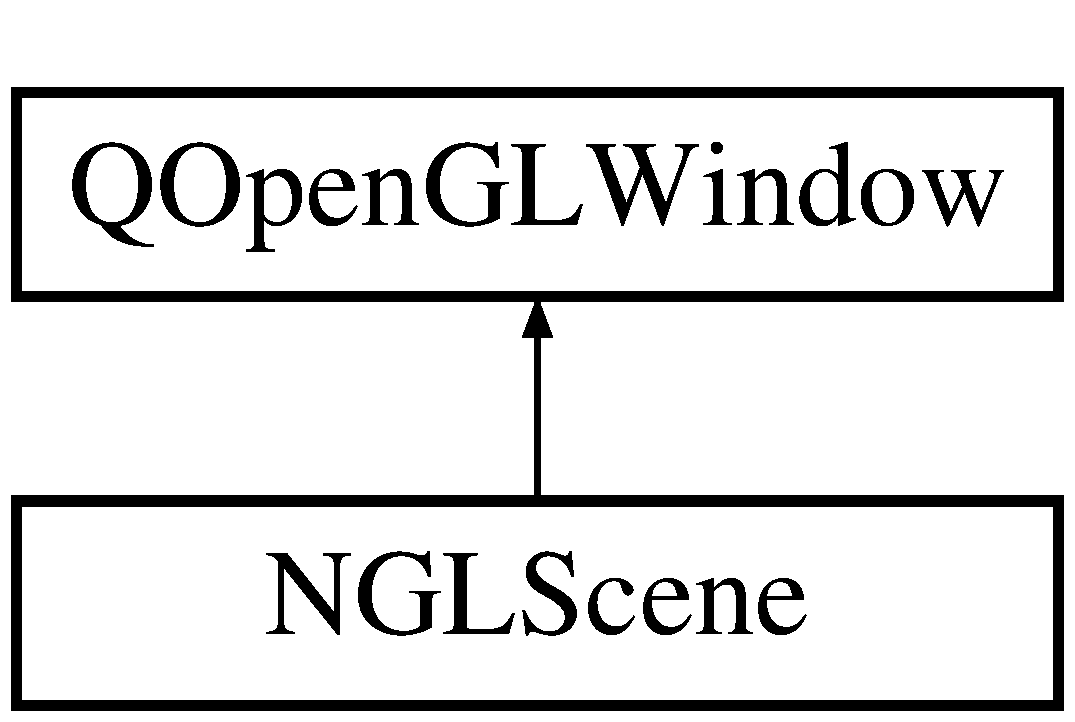
\includegraphics[height=2.000000cm]{classNGLScene}
\end{center}
\end{figure}
\subsection*{Public Member Functions}
\begin{DoxyCompactItemize}
\item 
\hyperlink{classNGLScene_a1bed6be9823459aeb1e58af2464ba633}{N\+G\+L\+Scene} ()
\begin{DoxyCompactList}\small\item\em ctor for our N\+GL drawing class \end{DoxyCompactList}\item 
\hyperlink{classNGLScene_abda05d130945833bfbb6bad8d619f7f5}{$\sim$\+N\+G\+L\+Scene} ()\hypertarget{classNGLScene_abda05d130945833bfbb6bad8d619f7f5}{}\label{classNGLScene_abda05d130945833bfbb6bad8d619f7f5}

\begin{DoxyCompactList}\small\item\em dtor must close down ngl and release Open\+GL resources \end{DoxyCompactList}\item 
void \hyperlink{classNGLScene_aab2b866db534d286a56cc2240ed98790}{initialize\+GL} ()\hypertarget{classNGLScene_aab2b866db534d286a56cc2240ed98790}{}\label{classNGLScene_aab2b866db534d286a56cc2240ed98790}

\begin{DoxyCompactList}\small\item\em the initialize class is called once when the window is created and we have a valid GL context use this to setup any default GL stuff \end{DoxyCompactList}\item 
void \hyperlink{classNGLScene_a37bec65bfba7b7a717d803d369221e2d}{paint\+GL} ()\hypertarget{classNGLScene_a37bec65bfba7b7a717d803d369221e2d}{}\label{classNGLScene_a37bec65bfba7b7a717d803d369221e2d}

\begin{DoxyCompactList}\small\item\em this is called everytime we want to draw the scene \end{DoxyCompactList}\end{DoxyCompactItemize}


\subsection{Detailed Description}
our main glwindow widget for N\+GL applications all drawing elements are put in this file 

\subsection{Constructor \& Destructor Documentation}
\index{N\+G\+L\+Scene@{N\+G\+L\+Scene}!N\+G\+L\+Scene@{N\+G\+L\+Scene}}
\index{N\+G\+L\+Scene@{N\+G\+L\+Scene}!N\+G\+L\+Scene@{N\+G\+L\+Scene}}
\subsubsection[{\texorpdfstring{N\+G\+L\+Scene()}{NGLScene()}}]{\setlength{\rightskip}{0pt plus 5cm}N\+G\+L\+Scene\+::\+N\+G\+L\+Scene (
\begin{DoxyParamCaption}
{}
\end{DoxyParamCaption}
)}\hypertarget{classNGLScene_a1bed6be9823459aeb1e58af2464ba633}{}\label{classNGLScene_a1bed6be9823459aeb1e58af2464ba633}


ctor for our N\+GL drawing class 


\begin{DoxyParams}[1]{Parameters}
\mbox{\tt in}  & {\em parent} & the parent window to the class \\
\hline
\end{DoxyParams}


The documentation for this class was generated from the following files\+:\begin{DoxyCompactItemize}
\item 
include/\hyperlink{NGLScene_8h}{N\+G\+L\+Scene.\+h}\item 
src/N\+G\+L\+Scene.\+cpp\end{DoxyCompactItemize}

\hypertarget{classNNS}{}\section{N\+NS Class Reference}
\label{classNNS}\index{N\+NS@{N\+NS}}


Uniform grid implementation that creates the grid map and builds neighbor tables for each particle, neighbor table parallelised.  




{\ttfamily \#include $<$N\+N\+S.\+h$>$}

\subsection*{Public Member Functions}
\begin{DoxyCompactItemize}
\item 
\hyperlink{classNNS_abade6f586869c6bfdac7c05eeaf50d9c}{N\+NS} ()\hypertarget{classNNS_abade6f586869c6bfdac7c05eeaf50d9c}{}\label{classNNS_abade6f586869c6bfdac7c05eeaf50d9c}

\begin{DoxyCompactList}\small\item\em \hyperlink{classNNS}{N\+NS} Default ctor. \end{DoxyCompactList}\item 
\hyperlink{classNNS_a1d4eddea97d0ab3e7a2527b0c2bd39df}{$\sim$\+N\+NS} ()\hypertarget{classNNS_a1d4eddea97d0ab3e7a2527b0c2bd39df}{}\label{classNNS_a1d4eddea97d0ab3e7a2527b0c2bd39df}

\begin{DoxyCompactList}\small\item\em $\sim$\+N\+NS Default dtor \end{DoxyCompactList}\item 
void \hyperlink{classNNS_ad05c2587ca92a0d6d424383aca42a9b6}{init} (const \hyperlink{classBoundingBox}{Bounding\+Box} \&\+\_\+bb, const unsigned int \&\+\_\+particle\+Count, const unsigned int \&\+\_\+max\+Neighbors=60)
\begin{DoxyCompactList}\small\item\em init Method to initialise the grid and prepare it for the nns \end{DoxyCompactList}\item 
void \hyperlink{classNNS_a69702190a37743cb666da72c9828fb61}{build\+Table} (const std\+::vector$<$ \hyperlink{structParticle}{Particle} $\ast$ $>$ \&\+\_\+particles)
\begin{DoxyCompactList}\small\item\em build\+Table Builds the grid and constructs the neighbor table for each particle \end{DoxyCompactList}\item 
void \hyperlink{classNNS_af7b3f89428efe4016240c595ce66d500}{clean\+Table} ()\hypertarget{classNNS_af7b3f89428efe4016240c595ce66d500}{}\label{classNNS_af7b3f89428efe4016240c595ce66d500}

\begin{DoxyCompactList}\small\item\em clean\+Table Cleans the grid and neighbor tables \end{DoxyCompactList}\item 
std\+::pair$<$ unsigned int $\ast$, unsigned int $>$ \hyperlink{classNNS_a70bef5d583a31d9af81a72d529152a89}{get\+Neighbors} (const int \&\+\_\+pid)
\begin{DoxyCompactList}\small\item\em get\+Neighbors Method to get the neighbors of a particle \end{DoxyCompactList}\end{DoxyCompactItemize}


\subsection{Detailed Description}
Uniform grid implementation that creates the grid map and builds neighbor tables for each particle, neighbor table parallelised. 

\subsection{Member Function Documentation}
\index{N\+NS@{N\+NS}!build\+Table@{build\+Table}}
\index{build\+Table@{build\+Table}!N\+NS@{N\+NS}}
\subsubsection[{\texorpdfstring{build\+Table(const std\+::vector$<$ Particle $\ast$ $>$ \&\+\_\+particles)}{buildTable(const std::vector< Particle * > &_particles)}}]{\setlength{\rightskip}{0pt plus 5cm}void N\+N\+S\+::build\+Table (
\begin{DoxyParamCaption}
\item[{const std\+::vector$<$ {\bf Particle} $\ast$ $>$ \&}]{\+\_\+particles}
\end{DoxyParamCaption}
)}\hypertarget{classNNS_a69702190a37743cb666da72c9828fb61}{}\label{classNNS_a69702190a37743cb666da72c9828fb61}


build\+Table Builds the grid and constructs the neighbor table for each particle 


\begin{DoxyParams}[1]{Parameters}
\mbox{\tt in}  & {\em \+\_\+particles} & Vector containing the particles \\
\hline
\end{DoxyParams}
\index{N\+NS@{N\+NS}!get\+Neighbors@{get\+Neighbors}}
\index{get\+Neighbors@{get\+Neighbors}!N\+NS@{N\+NS}}
\subsubsection[{\texorpdfstring{get\+Neighbors(const int \&\+\_\+pid)}{getNeighbors(const int &_pid)}}]{\setlength{\rightskip}{0pt plus 5cm}std\+::pair$<$ unsigned int $\ast$, unsigned int $>$ N\+N\+S\+::get\+Neighbors (
\begin{DoxyParamCaption}
\item[{const int \&}]{\+\_\+pid}
\end{DoxyParamCaption}
)}\hypertarget{classNNS_a70bef5d583a31d9af81a72d529152a89}{}\label{classNNS_a70bef5d583a31d9af81a72d529152a89}


get\+Neighbors Method to get the neighbors of a particle 


\begin{DoxyParams}[1]{Parameters}
\mbox{\tt in}  & {\em \+\_\+pid} & Index of the particle in question \\
\hline
\end{DoxyParams}
\begin{DoxyReturn}{Returns}
Pair containing the pointer to the neighbor table of the particle and the amount of neighbors 
\end{DoxyReturn}
\index{N\+NS@{N\+NS}!init@{init}}
\index{init@{init}!N\+NS@{N\+NS}}
\subsubsection[{\texorpdfstring{init(const Bounding\+Box \&\+\_\+bb, const unsigned int \&\+\_\+particle\+Count, const unsigned int \&\+\_\+max\+Neighbors=60)}{init(const BoundingBox &_bb, const unsigned int &_particleCount, const unsigned int &_maxNeighbors=60)}}]{\setlength{\rightskip}{0pt plus 5cm}void N\+N\+S\+::init (
\begin{DoxyParamCaption}
\item[{const {\bf Bounding\+Box} \&}]{\+\_\+bb, }
\item[{const unsigned int \&}]{\+\_\+particle\+Count, }
\item[{const unsigned int \&}]{\+\_\+max\+Neighbors = {\ttfamily 60}}
\end{DoxyParamCaption}
)}\hypertarget{classNNS_ad05c2587ca92a0d6d424383aca42a9b6}{}\label{classNNS_ad05c2587ca92a0d6d424383aca42a9b6}


init Method to initialise the grid and prepare it for the nns 


\begin{DoxyParams}[1]{Parameters}
\mbox{\tt in}  & {\em \+\_\+bb} & Bounding box of the simulation \\
\hline
\mbox{\tt in}  & {\em \+\_\+particle\+Count} & \hyperlink{structParticle}{Particle} count \\
\hline
\mbox{\tt in}  & {\em \+\_\+max\+Neighbors} & Max neighbors per particle (if exceeded, the particles will be ignored) \\
\hline
\end{DoxyParams}


The documentation for this class was generated from the following files\+:\begin{DoxyCompactItemize}
\item 
include/\hyperlink{NNS_8h}{N\+N\+S.\+h}\item 
src/N\+N\+S.\+cpp\end{DoxyCompactItemize}

\hypertarget{structParticle}{}\section{Particle Struct Reference}
\label{structParticle}\index{Particle@{Particle}}


Simple particle struct holding the position, velocity etc.  




{\ttfamily \#include $<$Particle.\+h$>$}

\subsection*{Public Member Functions}
\begin{DoxyCompactItemize}
\item 
\hyperlink{structParticle_ac27e166117e21a32c2a0dfe4bd6fd8bd}{Particle} (const float \&\+\_\+x=0.f, const float \&\+\_\+y=0.f, const float \&\+\_\+z=0.f, const float \&\+\_\+r=0.\+125f)
\begin{DoxyCompactList}\small\item\em \hyperlink{structParticle}{Particle} Default ctor. \end{DoxyCompactList}\end{DoxyCompactItemize}
\subsection*{Public Attributes}
\begin{DoxyCompactItemize}
\item 
ngl\+::\+Vec3 \hyperlink{structParticle_a2b5ef8d7207002ec8e887492a5bbe9f2}{m\+\_\+pos}\hypertarget{structParticle_a2b5ef8d7207002ec8e887492a5bbe9f2}{}\label{structParticle_a2b5ef8d7207002ec8e887492a5bbe9f2}

\begin{DoxyCompactList}\small\item\em m\+\_\+pos Position of a particle \end{DoxyCompactList}\item 
ngl\+::\+Vec3 \hyperlink{structParticle_a07d3e906cc3a72402264eef170928dc2}{m\+\_\+pred\+Pos}\hypertarget{structParticle_a07d3e906cc3a72402264eef170928dc2}{}\label{structParticle_a07d3e906cc3a72402264eef170928dc2}

\begin{DoxyCompactList}\small\item\em m\+\_\+pred\+Pos Predicted position of a particle \end{DoxyCompactList}\item 
ngl\+::\+Vec3 \hyperlink{structParticle_a0193dd643fac3bea35449487b6a01bb8}{m\+\_\+pos\+Update}\hypertarget{structParticle_a0193dd643fac3bea35449487b6a01bb8}{}\label{structParticle_a0193dd643fac3bea35449487b6a01bb8}

\begin{DoxyCompactList}\small\item\em m\+\_\+pos\+Update Calculated position update of a particle \end{DoxyCompactList}\item 
ngl\+::\+Vec3 \hyperlink{structParticle_a4098b3ed1500b5994784b1de15d19b34}{m\+\_\+vel}\hypertarget{structParticle_a4098b3ed1500b5994784b1de15d19b34}{}\label{structParticle_a4098b3ed1500b5994784b1de15d19b34}

\begin{DoxyCompactList}\small\item\em m\+\_\+vel Velocity of a particle \end{DoxyCompactList}\item 
ngl\+::\+Vec3 \hyperlink{structParticle_a71714f50096808645b525a035d1109cc}{m\+\_\+ext\+Forces}\hypertarget{structParticle_a71714f50096808645b525a035d1109cc}{}\label{structParticle_a71714f50096808645b525a035d1109cc}

\begin{DoxyCompactList}\small\item\em m\+\_\+ext\+Forces External forces to a particle \end{DoxyCompactList}\item 
ngl\+::\+Vec4 \hyperlink{structParticle_a28fb9bc37248c0463a84fe1a302bfb18}{m\+\_\+colour}\hypertarget{structParticle_a28fb9bc37248c0463a84fe1a302bfb18}{}\label{structParticle_a28fb9bc37248c0463a84fe1a302bfb18}

\begin{DoxyCompactList}\small\item\em m\+\_\+colour Colour of a particle \end{DoxyCompactList}\item 
float \hyperlink{structParticle_ab78b76aeb4d163132a0c27ea4c5beb75}{m\+\_\+mass}\hypertarget{structParticle_ab78b76aeb4d163132a0c27ea4c5beb75}{}\label{structParticle_ab78b76aeb4d163132a0c27ea4c5beb75}

\begin{DoxyCompactList}\small\item\em m\+\_\+mass Mass of a particle \end{DoxyCompactList}\item 
float \hyperlink{structParticle_af6aee0d324572f74a1bdc28937d04a0b}{m\+\_\+radius}\hypertarget{structParticle_af6aee0d324572f74a1bdc28937d04a0b}{}\label{structParticle_af6aee0d324572f74a1bdc28937d04a0b}

\begin{DoxyCompactList}\small\item\em m\+\_\+radius Radius of a particle \end{DoxyCompactList}\item 
float \hyperlink{structParticle_a7ef5758b3dbc3ea263b670012f0c2fe5}{m\+\_\+density}\hypertarget{structParticle_a7ef5758b3dbc3ea263b670012f0c2fe5}{}\label{structParticle_a7ef5758b3dbc3ea263b670012f0c2fe5}

\begin{DoxyCompactList}\small\item\em m\+\_\+density Density of a particle \end{DoxyCompactList}\item 
float \hyperlink{structParticle_a253dea0d4438cac9831c22f75c2b8163}{m\+\_\+lambda}\hypertarget{structParticle_a253dea0d4438cac9831c22f75c2b8163}{}\label{structParticle_a253dea0d4438cac9831c22f75c2b8163}

\begin{DoxyCompactList}\small\item\em m\+\_\+lambda Scaling factor of a particle \end{DoxyCompactList}\end{DoxyCompactItemize}


\subsection{Detailed Description}
Simple particle struct holding the position, velocity etc. 

\subsection{Constructor \& Destructor Documentation}
\index{Particle@{Particle}!Particle@{Particle}}
\index{Particle@{Particle}!Particle@{Particle}}
\subsubsection[{\texorpdfstring{Particle(const float \&\+\_\+x=0.\+f, const float \&\+\_\+y=0.\+f, const float \&\+\_\+z=0.\+f, const float \&\+\_\+r=0.\+125f)}{Particle(const float &_x=0.f, const float &_y=0.f, const float &_z=0.f, const float &_r=0.125f)}}]{\setlength{\rightskip}{0pt plus 5cm}Particle\+::\+Particle (
\begin{DoxyParamCaption}
\item[{const float \&}]{\+\_\+x = {\ttfamily 0.f}, }
\item[{const float \&}]{\+\_\+y = {\ttfamily 0.f}, }
\item[{const float \&}]{\+\_\+z = {\ttfamily 0.f}, }
\item[{const float \&}]{\+\_\+r = {\ttfamily 0.125f}}
\end{DoxyParamCaption}
)\hspace{0.3cm}{\ttfamily [inline]}}\hypertarget{structParticle_ac27e166117e21a32c2a0dfe4bd6fd8bd}{}\label{structParticle_ac27e166117e21a32c2a0dfe4bd6fd8bd}


\hyperlink{structParticle}{Particle} Default ctor. 


\begin{DoxyParams}[1]{Parameters}
\mbox{\tt in}  & {\em \+\_\+x} & Initial x-\/position \\
\hline
\mbox{\tt in}  & {\em \+\_\+y} & Initial y-\/position \\
\hline
\mbox{\tt in}  & {\em \+\_\+z} & Initial z-\/position \\
\hline
\mbox{\tt in}  & {\em \+\_\+r} & Radius of the particle \\
\hline
\end{DoxyParams}


The documentation for this struct was generated from the following file\+:\begin{DoxyCompactItemize}
\item 
include/\hyperlink{Particle_8h}{Particle.\+h}\end{DoxyCompactItemize}

\hypertarget{structWall}{}\section{Wall Struct Reference}
\label{structWall}\index{Wall@{Wall}}


Simple wall structure containing the center point, normal of the wall.  




{\ttfamily \#include $<$Bounding\+Box.\+h$>$}

\subsection*{Public Attributes}
\begin{DoxyCompactItemize}
\item 
ngl\+::\+Vec3 {\bfseries centre}\hypertarget{structWall_aee57d6158d6d7380839d9615cd149deb}{}\label{structWall_aee57d6158d6d7380839d9615cd149deb}

\item 
ngl\+::\+Vec3 {\bfseries normal}\hypertarget{structWall_a001549604fc2b6d526c814d17eeb7e81}{}\label{structWall_a001549604fc2b6d526c814d17eeb7e81}

\item 
float {\bfseries d}\hypertarget{structWall_a2e62214f52d96f5e2516be239a6702f3}{}\label{structWall_a2e62214f52d96f5e2516be239a6702f3}

\end{DoxyCompactItemize}


\subsection{Detailed Description}
Simple wall structure containing the center point, normal of the wall. 

The documentation for this struct was generated from the following file\+:\begin{DoxyCompactItemize}
\item 
include/\hyperlink{BoundingBox_8h}{Bounding\+Box.\+h}\end{DoxyCompactItemize}

\chapter{File Documentation}
\hypertarget{BoundingBox_8h}{}\section{include/\+Bounding\+Box.h File Reference}
\label{BoundingBox_8h}\index{include/\+Bounding\+Box.\+h@{include/\+Bounding\+Box.\+h}}


Implementation of a simple \hyperlink{classBoundingBox}{Bounding\+Box} used as the boundaries of the simulation.  


{\ttfamily \#include $<$memory$>$}\\*
{\ttfamily \#include $<$ngl/\+Vertex\+Array\+Object.\+h$>$}\\*
{\ttfamily \#include $<$ngl/\+Vec3.\+h$>$}\\*
\subsection*{Classes}
\begin{DoxyCompactItemize}
\item 
struct \hyperlink{structWall}{Wall}
\begin{DoxyCompactList}\small\item\em Simple wall structure containing the center point, normal of the wall. \end{DoxyCompactList}\item 
class \hyperlink{classBoundingBox}{Bounding\+Box}
\begin{DoxyCompactList}\small\item\em Simple \hyperlink{classBoundingBox}{Bounding\+Box} class to work as the boundaries of the simulation. \end{DoxyCompactList}\end{DoxyCompactItemize}
\subsection*{Typedefs}
\begin{DoxyCompactItemize}
\item 
typedef struct \hyperlink{structWall}{Wall} {\bfseries Wall}\hypertarget{BoundingBox_8h_ab87ac498e0587de73a41a7af295978ad}{}\label{BoundingBox_8h_ab87ac498e0587de73a41a7af295978ad}

\end{DoxyCompactItemize}


\subsection{Detailed Description}
Implementation of a simple \hyperlink{classBoundingBox}{Bounding\+Box} used as the boundaries of the simulation. 

\begin{DoxyAuthor}{Author}
Teemu Lindborg 
\end{DoxyAuthor}
\begin{DoxyVersion}{Version}
1.\+0 
\end{DoxyVersion}
\begin{DoxyDate}{Date}
17.\+03.\+2016 Commented Revision History \+: Initial version 15.\+02.\+2016 
\end{DoxyDate}
\begin{DoxyRefDesc}{Todo}
\item[\hyperlink{todo__todo000001}{Todo}]Add the possibility to define each corner point for non axis-\/aligned boxes. \end{DoxyRefDesc}

\hypertarget{FluidSolver_8h}{}\section{include/\+Fluid\+Solver.h File Reference}
\label{FluidSolver_8h}\index{include/\+Fluid\+Solver.\+h@{include/\+Fluid\+Solver.\+h}}


Position Based Fluids solver class, based on the paper \href{http://mmacklin.com/pbf_sig_preprint.pdf}{\tt http\+://mmacklin.\+com/pbf\+\_\+sig\+\_\+preprint.\+pdf}.  


{\ttfamily \#include $<$ngl/\+Vec3.\+h$>$}\\*
{\ttfamily \#include $<$vector$>$}\\*
{\ttfamily \#include \char`\"{}Particle.\+h\char`\"{}}\\*
\subsection*{Classes}
\begin{DoxyCompactItemize}
\item 
class \hyperlink{classFluidSolver}{Fluid\+Solver}
\begin{DoxyCompactList}\small\item\em Solver implementing the algorithm defined in the original P\+BF paper by M. Macklin \& M. Müller. \end{DoxyCompactList}\end{DoxyCompactItemize}
\subsection*{Variables}
\begin{DoxyCompactItemize}
\item 
constexpr float {\bfseries m\+\_\+pi} = 3.\+14159265359f\hypertarget{FluidSolver_8h_a111957313cb1de6b13dfb8d5598c018d}{}\label{FluidSolver_8h_a111957313cb1de6b13dfb8d5598c018d}

\end{DoxyCompactItemize}


\subsection{Detailed Description}
Position Based Fluids solver class, based on the paper \href{http://mmacklin.com/pbf_sig_preprint.pdf}{\tt http\+://mmacklin.\+com/pbf\+\_\+sig\+\_\+preprint.\+pdf}. 

\begin{DoxyAuthor}{Author}
Teemu Lindborg 
\end{DoxyAuthor}
\begin{DoxyVersion}{Version}
1.\+0 
\end{DoxyVersion}
\begin{DoxyDate}{Date}
18.\+03.\+2016 Commenting and tidying up Revision History \+: Started blocking out 08.\+02.\+16 Implemented the solver and commented the code 17.\+03.\+16 
\end{DoxyDate}
\begin{DoxyRefDesc}{Todo}
\item[\hyperlink{todo__todo000002}{Todo}]Make the code more robust \end{DoxyRefDesc}

\hypertarget{FluidSystem_8h}{}\section{include/\+Fluid\+System.h File Reference}
\label{FluidSystem_8h}\index{include/\+Fluid\+System.\+h@{include/\+Fluid\+System.\+h}}


Fluid system -\/class encapsulates and plugs together the whole system, handles the creation of the particles and calls the correct member classes/methods to build a functioning fluid system.  


{\ttfamily \#include $<$memory$>$}\\*
{\ttfamily \#include $<$vector$>$}\\*
{\ttfamily \#include \char`\"{}Bounding\+Box.\+h\char`\"{}}\\*
{\ttfamily \#include \char`\"{}Fluid\+Solver.\+h\char`\"{}}\\*
{\ttfamily \#include \char`\"{}N\+N\+S.\+h\char`\"{}}\\*
{\ttfamily \#include \char`\"{}Particle.\+h\char`\"{}}\\*
\subsection*{Classes}
\begin{DoxyCompactItemize}
\item 
class \hyperlink{classFluidSystem}{Fluid\+System}
\begin{DoxyCompactList}\small\item\em Class creating the particles and bringing together the solver and grid. \end{DoxyCompactList}\end{DoxyCompactItemize}


\subsection{Detailed Description}
Fluid system -\/class encapsulates and plugs together the whole system, handles the creation of the particles and calls the correct member classes/methods to build a functioning fluid system. 

\begin{DoxyAuthor}{Author}
Teemu Lindborg 
\end{DoxyAuthor}
\begin{DoxyVersion}{Version}
1.\+0 
\end{DoxyVersion}
\begin{DoxyDate}{Date}
17/03/2016 Commenting and tidying up Revision History \+: Started blocking out 08/02/16 Implemented the system and commented code -\/17/03/2016 
\end{DoxyDate}
\begin{DoxyRefDesc}{Todo}
\item[\hyperlink{todo__todo000003}{Todo}]Implement a G\+UI to run the variables in the system \end{DoxyRefDesc}

\hypertarget{NGLScene_8h}{}\section{include/\+N\+G\+L\+Scene.h File Reference}
\label{NGLScene_8h}\index{include/\+N\+G\+L\+Scene.\+h@{include/\+N\+G\+L\+Scene.\+h}}


this class inherits from the Qt Open\+G\+L\+Window and allows us to use N\+GL to draw Open\+GL  


{\ttfamily \#include $<$ngl/\+Camera.\+h$>$}\\*
{\ttfamily \#include $<$ngl/\+Colour.\+h$>$}\\*
{\ttfamily \#include $<$ngl/\+Light.\+h$>$}\\*
{\ttfamily \#include $<$ngl/\+Transformation.\+h$>$}\\*
{\ttfamily \#include $<$ngl/\+Text.\+h$>$}\\*
{\ttfamily \#include $<$Q\+Open\+G\+L\+Window$>$}\\*
{\ttfamily \#include $<$chrono$>$}\\*
{\ttfamily \#include \char`\"{}Fluid\+System.\+h\char`\"{}}\\*
\subsection*{Classes}
\begin{DoxyCompactItemize}
\item 
class \hyperlink{classNGLScene}{N\+G\+L\+Scene}
\begin{DoxyCompactList}\small\item\em our main glwindow widget for N\+GL applications all drawing elements are put in this file \end{DoxyCompactList}\end{DoxyCompactItemize}


\subsection{Detailed Description}
this class inherits from the Qt Open\+G\+L\+Window and allows us to use N\+GL to draw Open\+GL 

\begin{DoxyAuthor}{Author}
Jonathan Macey 
\end{DoxyAuthor}
\begin{DoxyVersion}{Version}
1.\+0 
\end{DoxyVersion}
\begin{DoxyDate}{Date}
10/9/13 Revision History \+: This is an initial version used for the new N\+G\+L6 / Qt 5 demos 
\end{DoxyDate}

\hypertarget{NNS_8h}{}\section{include/\+N\+NS.h File Reference}
\label{NNS_8h}\index{include/\+N\+N\+S.\+h@{include/\+N\+N\+S.\+h}}


Nearest neighbor searching class using a uniform grid where the grid size is based on the particle diameter.  


{\ttfamily \#include $<$unordered\+\_\+map$>$}\\*
{\ttfamily \#include \char`\"{}Bounding\+Box.\+h\char`\"{}}\\*
{\ttfamily \#include \char`\"{}Particle.\+h\char`\"{}}\\*
\subsection*{Classes}
\begin{DoxyCompactItemize}
\item 
class \hyperlink{classNNS}{N\+NS}
\begin{DoxyCompactList}\small\item\em Uniform grid implementation that creates the grid map and builds neighbor tables for each particle, neighbor table parallelised. \end{DoxyCompactList}\end{DoxyCompactItemize}


\subsection{Detailed Description}
Nearest neighbor searching class using a uniform grid where the grid size is based on the particle diameter. 

\begin{DoxyAuthor}{Author}
Teemu Lindborg 
\end{DoxyAuthor}
\begin{DoxyVersion}{Version}
1.\+0 
\end{DoxyVersion}
\begin{DoxyDate}{Date}
17/03/2016 Commenting and tidying up Revision History \+: Started blocking out 08/02/2016 Implemented the grid and nearest neighbor searching ...-\/17/03/2016 
\end{DoxyDate}
\begin{DoxyRefDesc}{Todo}
\item[\hyperlink{todo__todo000004}{Todo}]Research and implement a more efficient way \end{DoxyRefDesc}

\hypertarget{Particle_8h}{}\section{include/\+Particle.h File Reference}
\label{Particle_8h}\index{include/\+Particle.\+h@{include/\+Particle.\+h}}


Simple particle struct.  


{\ttfamily \#include $<$vector$>$}\\*
{\ttfamily \#include $<$ngl/\+Vec4.\+h$>$}\\*
\subsection*{Classes}
\begin{DoxyCompactItemize}
\item 
struct \hyperlink{structParticle}{Particle}
\begin{DoxyCompactList}\small\item\em Simple particle struct holding the position, velocity etc. \end{DoxyCompactList}\end{DoxyCompactItemize}
\subsection*{Typedefs}
\begin{DoxyCompactItemize}
\item 
typedef struct \hyperlink{structParticle}{Particle} {\bfseries Particle}\hypertarget{Particle_8h_aeaa4f715238c24bf147c7af545845701}{}\label{Particle_8h_aeaa4f715238c24bf147c7af545845701}

\end{DoxyCompactItemize}


\subsection{Detailed Description}
Simple particle struct. 

\begin{DoxyAuthor}{Author}
Teemu Lindborg 
\end{DoxyAuthor}
\begin{DoxyVersion}{Version}
1.\+0 
\end{DoxyVersion}
\begin{DoxyDate}{Date}
08/02/16 Initial blocking Revision History \+: Started blocking out 08/02/16 
\end{DoxyDate}
\begin{DoxyRefDesc}{Todo}
\item[\hyperlink{todo__todo000005}{Todo}]Refining \end{DoxyRefDesc}

%--- End generated contents ---

% Index
\backmatter
\newpage
\phantomsection
\clearemptydoublepage
\addcontentsline{toc}{chapter}{Index}
\printindex

\end{document}
